% Owner: D. Event-started SIR; supersedes the observation-start experiment.
\paragraph{Event-driven SIR (M3c).}\label{sec:d_sir}
Each network uses 200 seeds at randomly selected events in its first 70\% of event
positions. CM seeds use the sender; PS randomly selects either endpoint. The selected
seed event itself is excluded by the strict-time convention. Infectious duration is
fixed, transmission probability is per record, and recovered nodes remain immune.
Final size includes the seed. A major outbreak reaches at least 5\% of period nodes.
Peak delays are averaged over major outbreaks only; $T_{\rm real}/\overline T_{\rm null}$
is a conditional ratio of means. Nulls with no major outbreaks give an undefined peak,
not a zero delay. Simultaneous infections and recoveries are grouped before measuring
prevalence; the earliest maximum is selected.
\begin{table*}[!htbp]\centering\small
\begin{tabular}{@{}llrrrrrrrr@{}}
\toprule & & \multicolumn{3}{c}{Final infected fraction} & \multicolumn{3}{c}{Major outbreak probability} & \multicolumn{2}{c}{Peak ratio} \\
Dataset & $(\beta,D)$ & Real & P1 & P2 & Real & P1 & P2 & vs P1 & vs P2 \\
\midrule
PS & (0.05, 4 h) & 0.629 & 0.776 & 0.823 & 0.860 & 0.908 & 0.920 & 1.160 & 1.214 \\
PS & (0.02, 4 h) & 0.373 & 0.420 & 0.559 & 0.700 & 0.754 & 0.778 & 1.000 & 1.088 \\
PS & (0.1, 4 h) & 0.734 & 0.893 & 0.918 & 0.910 & 0.960 & 0.973 & 1.311 & 1.340 \\
PS & (0.05, 1 h) & 0.373 & 0.634 & 0.674 & 0.745 & 0.844 & 0.852 & 1.021 & 1.265 \\
CM & (0.2, 336 h) & 0.256 & 0.250 & 0.276 & 0.825 & 0.791 & 0.799 & 0.888 & 0.995 \\
CM & (0.05, 336 h) & 0.026 & 0.013 & 0.025 & 0.215 & 0.082 & 0.192 & 0.934 & 0.991 \\
CM & (0.5, 336 h) & 0.460 & 0.506 & 0.530 & 0.975 & 0.954 & 0.965 & 0.924 & 0.982 \\
CM & (0.2, 72 h) & 0.074 & 0.043 & 0.066 & 0.555 & 0.342 & 0.428 & 0.720 & 1.013 \\
\bottomrule\end{tabular}
\caption{Four SIR settings per dataset, 200 seeds per network, 20 nulls per family.
The first setting in each dataset is primary. The peak-ratio population is restricted
to major outbreaks and can differ between real and null networks.}\label{tab:d-sir}
\end{table*}
\begin{figure*}[!htbp]
\centering
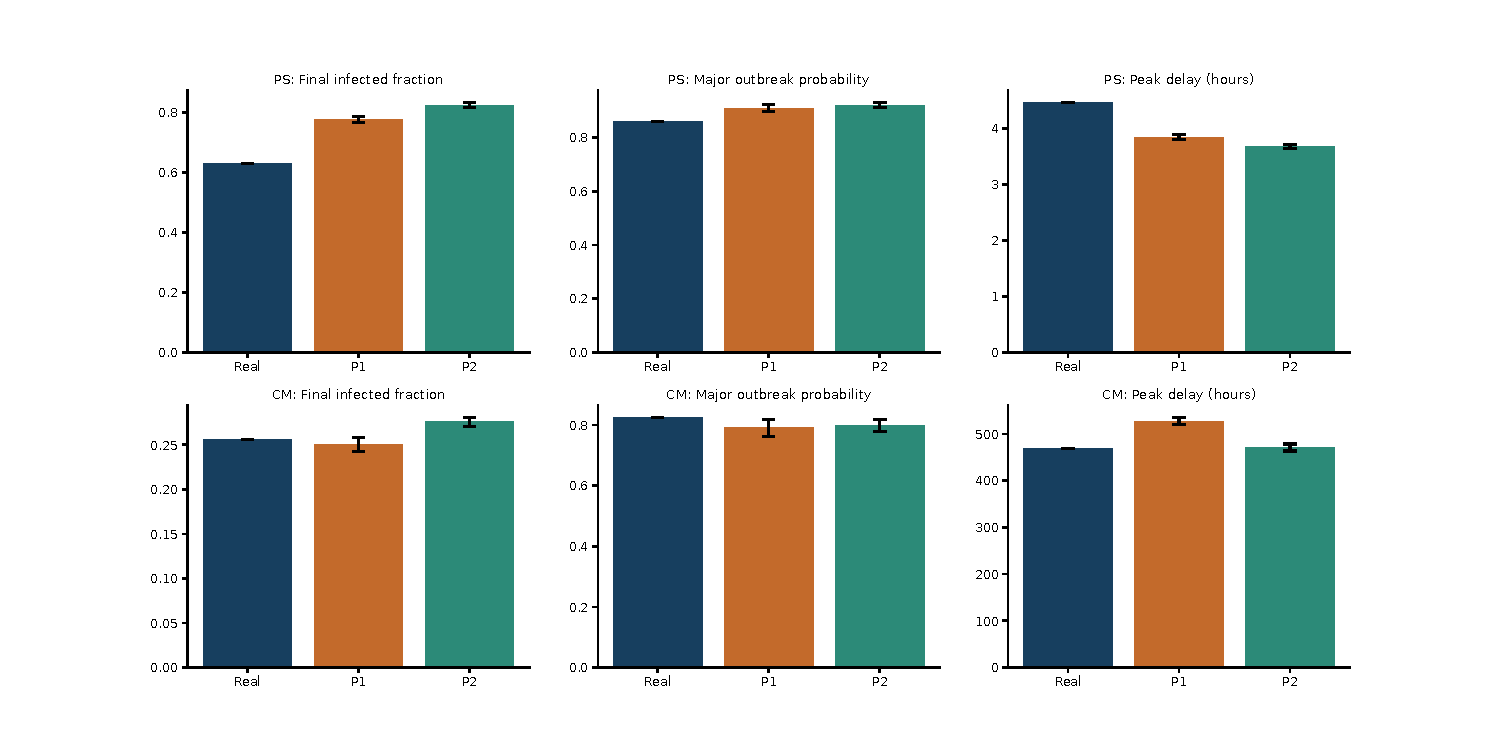
\includegraphics[width=\linewidth]{d_sir_event_seeds.pdf}
\caption{Primary SIR settings. Peak delay is conditional on major outbreaks; errors describe null-network variation.}
\label{fig:d_sir}
\end{figure*}
The revised design produces nontrivial CM outbreaks. Absence of secondary infections
in the earlier run arose from infecting seeds at the observation boundary with an
unsuitable short duration; it is not evidence for an intrinsic property of CM.

\paragraph{Parameter, null and outcome dependence.}
For PS versus P1, the peak ratio is 1.0005 at $\beta=.02$ (negligible peak difference),
1.160 at .05 and 1.311 at .10 for a four-hour infectious duration. Final size is
lower than both null families in all four tested settings; at the primary setting
it is 0.629 versus P1 0.776. The qualifying populations also differ: major outbreaks
occur for 0.860 of real seeds versus a mean 0.908 under P1. Conditional peak comparisons
therefore use different seed subsets and are not paired-seed causal slowdowns.

CM peaks earlier than P1 across the full-period settings (ratios 0.72--0.94),
whereas P2 peak ratios are approximately 0.98--1.01. Even the choice of timing
metric matters: at $\beta=.5$, 14 days, the peak ratio to P1 is 0.924 but the
half-final-size time ratio is 1.061. The latter is time to half of each trajectory's
own final infected count, not time to a common epidemic size. These opposing signs
exclude a general claim that the entire spreading process is faster or slower.
In CM's second half, two weaker settings have no major real outbreaks (undefined
peak ratios); the primary setting still has major-outbreak probability 0.360.

PS's real mean final fraction is 0.629 over the full interval versus 0.821/0.788
in the halves. Uniform sampling from the first 70\% of each event stream changes
seed identities, start positions and residual observation horizons when the interval
is split. Finite horizons and schedule boundaries may contribute; these CSV comparisons
alone do not identify their contribution separately. These are protocol sensitivities,
not evidence that truncating the data intrinsically strengthens propagation.
